\documentclass[10pt]{article}
\usepackage[utf8]{inputenc}
\usepackage[T1]{fontenc}
\usepackage{graphicx}
\usepackage[export]{adjustbox}
\graphicspath{ {./images/} }
\usepackage{amsmath}
\usepackage{amsfonts}
\usepackage{amssymb}
\usepackage[version=4]{mhchem}
\usepackage{stmaryrd}
\usepackage{caption}

\begin{document}


\section*{2 Galactic Surveys (105 points)}
In Cosmology, observations of the spatial distribution of galaxies are crucial to understanding the evolution and expansion of the Universe. Numerous telescopes conduct surveys to produce catalogues of galaxies, which are then subjected to statistical analysis. Usually, galaxies form in groups, which together are part of a cluster, surrounded by a very large, spherical dark-matter halo. Most of the matter is concentrated in the centre, thus there is a high probability of having a large-mass galaxy at the centre of the halo.\\
In this problem, we will assume that all halos have one central galaxy and several groups of satellite galaxies, and use statistical analysis to draw inferences about the spatial distribution of galaxies. In Figure 1, you can see six different possible probability densities (A-F) for distances between galaxies. On the X axis is the separation distance between galaxies (a), and on the Y axis is the probability density ( $f_{p}(a)$ ). The probability of the distance between a pair of galaxies being in the range $a$, to $a+\Delta a$ is given by

$$
P(a)=f_{p}(a) \Delta a
$$

Note that $f_{p}(a)$ may take values greater than 1 in some cases.

\begin{figure}[h]
\begin{center}
  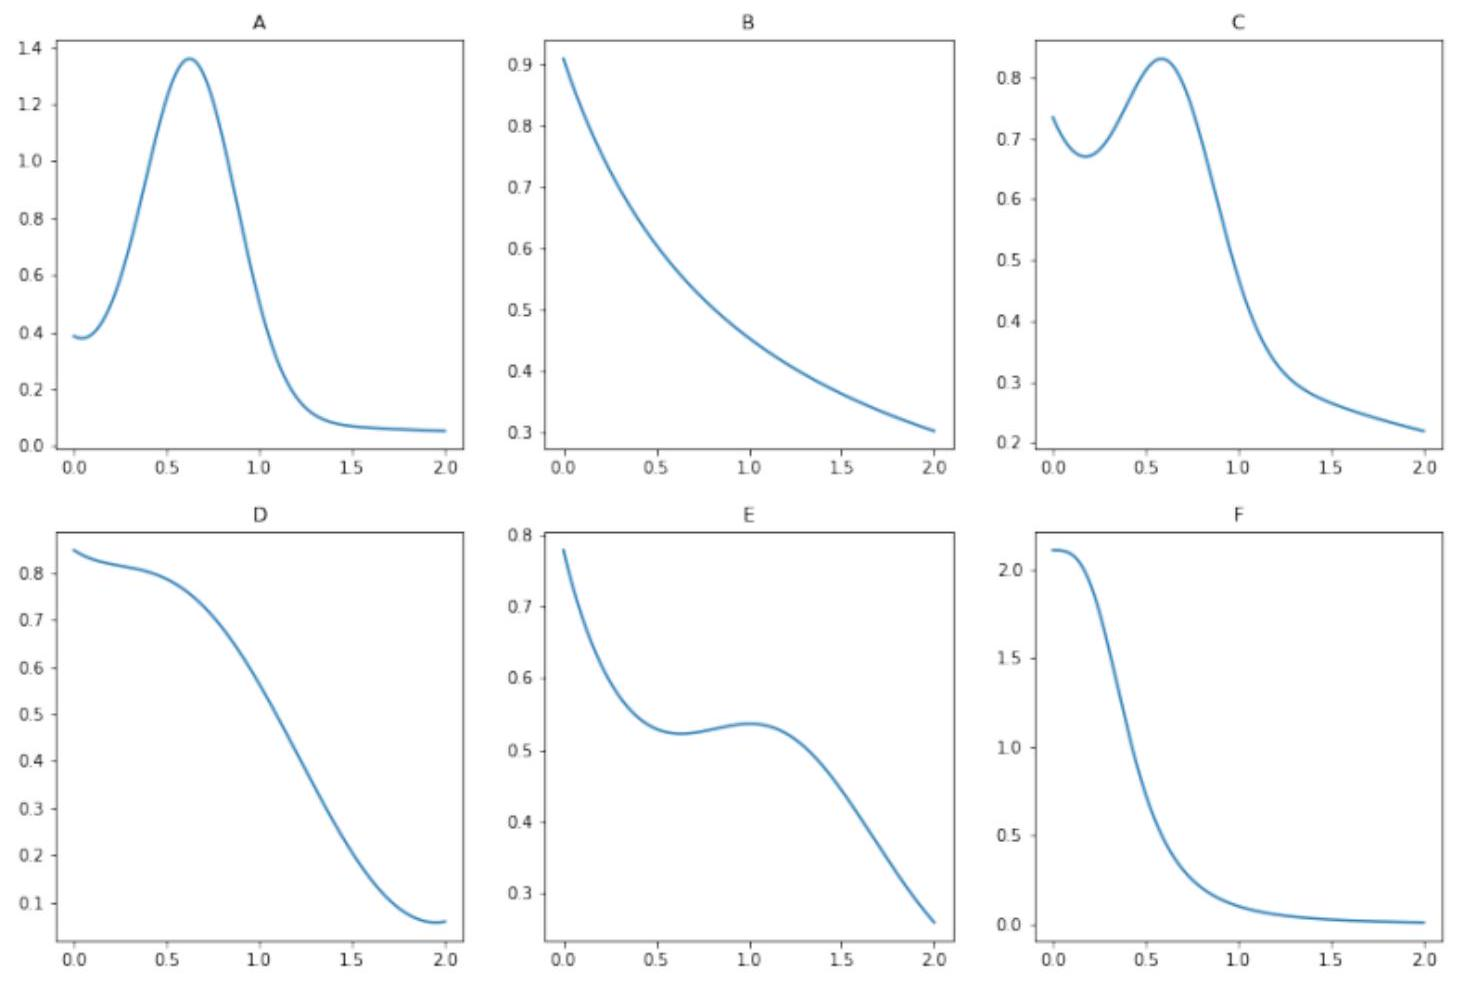
\includegraphics[width=\textwidth]{2025_09_11_3681df2e94a9f94ef296g-4}
\captionsetup{labelformat=empty}
\caption{Figure 1: Probability density of all possible galaxy pairs}
\end{center}
\end{figure}

\section*{Part 1 ( 60 pt )}
Table 1 gives the observational data of a single dark matter halo in the form of Cartesian coordinates of 16 satellite groups and the coordinates of the central galaxy which is given in the first row. $i^{\text {th }}$ group consists of $N_{i}$ galaxies. The origin of this coordinate system is the Earth. For simplicity we assume that a group of galaxies means a collection of galaxies with almost the same coordinates.

\begin{center}
\begin{tabular}{|l|l|l|l|l|}
\hline
i & $x$ (Mpc) & $y$ (Mpc) & $z$ (Mpc) & $N_{i}$ \\
\hline
C & 8.300 & 6.200 & 1.100 & Central \\
\hline
1 & 8.401 & 6.309 & 1.394 & 291 \\
\hline
2 & 9.883 & 7.189 & 1.506 & 170 \\
\hline
3 & 8.883 & 6.413 & 2.226 & 253 \\
\hline
4 & 8.444 & 6.569 & 2.439 & 8 \\
\hline
5 & 7.782 & 6.048 & -0.358 & 72 \\
\hline
6 & 8.780 & 6.305 & 2.463 & 120 \\
\hline
7 & 7.990 & 5.881 & 0.532 & 302 \\
\hline
8 & 8.540 & 6.388 & 0.369 & 52 \\
\hline
9 & 7.975 & 6.030 & 1.216 & 28 \\
\hline
10 & 7.072 & 5.431 & 0.488 & 40 \\
\hline
11 & 8.037 & 5.965 & 0.615 & 72 \\
\hline
12 & 8.681 & 6.483 & 0.734 & 379 \\
\hline
13 & 7.115 & 5.259 & 1.403 & 82 \\
\hline
14 & 9.587 & 7.130 & 0.322 & 62 \\
\hline
15 & 8.193 & 6.104 & 0.915 & 305 \\
\hline
16 & 7.613 & 5.847 & 1.666 & 293 \\
\hline
\end{tabular}
\end{center}

(a) The distribution of the satellite groups in $X-Z$ plane and $Y-Z$ plane has been plotted for you. Plot the distribution in the $X-Y$ plane on millimeter paper (6pt)\\
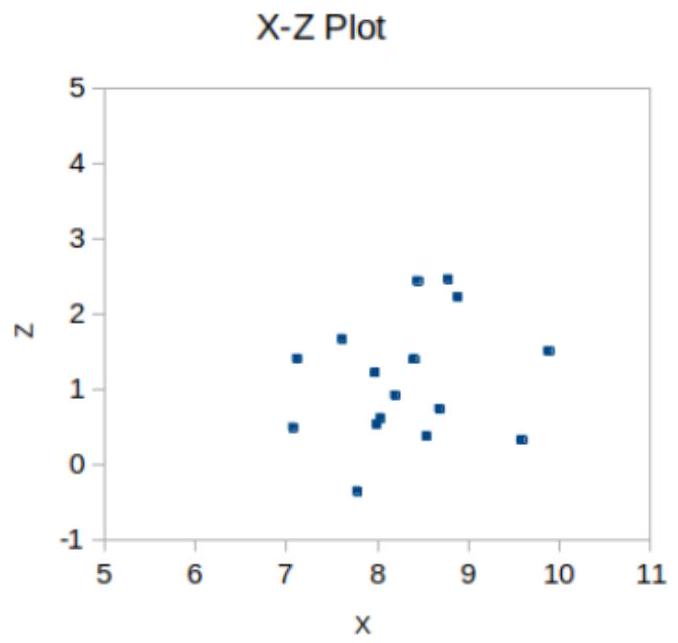
\includegraphics[max width=\textwidth, center]{2025_09_11_3681df2e94a9f94ef296g-5}\\
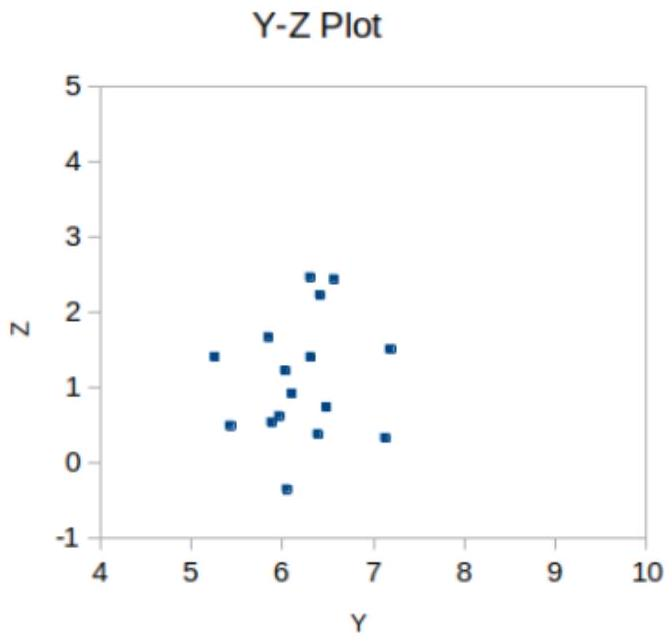
\includegraphics[max width=\textwidth, center]{2025_09_11_3681df2e94a9f94ef296g-5(1)}\\
(b) Given that this cluster of galaxies is shaped like a disk and our line of sight is in the plane of the disk, find the unit vector in the direction of the normal to the disk.\\
(c) Let us define a new coordinate system centered on the central galaxy, defining our line of sight from the Earth to the central galaxy as the $X^{\prime}$ axis and the normal to the disk as the $Z^{\prime}$ axis. Find the unit vectors for this coordinate system.\\
(d) Convert the given Cartesian coordinates to the new $X^{\prime} Y^{\prime} Z^{\prime}$ coordinates. Calculate $X^{\prime}, Y^{\prime}, Z^{\prime} . \quad(24 \mathrm{pt})$\\
(e) Write the equations necessary to convert the new $X^{\prime} Y^{\prime} Z^{\prime}$ ' Cartesian coordinates into spherical coordinates centered on the central galaxy. $\theta$ coordinate has been already calculated for you below. Calculate $R$ and $\phi$.

\begin{center}
\begin{tabular}{|r|c|}
\hline
i & $\theta$ \\
\hline\hline
1 & 1.652 \\
\hline
2 & 1.490 \\
\hline
3 & 1.432 \\
\hline
4 & 1.721 \\
\hline
5 & 1.692 \\
\hline
6 & 1.430 \\
\hline
7 & 1.474 \\
\hline
8 & 1.580 \\
\hline
9 & 1.723 \\
\hline
10 & 1.646 \\
\hline
11 & 1.519 \\
\hline
12 & 1.569 \\
\hline
13 & 1.542 \\
\hline
14 & 1.557 \\
\hline
15 & 1.516 \\
\hline
16 & 1.705 \\
\hline
\end{tabular}
\end{center}

Note: in spherical coordinates, one uses the coordinates $R, \theta$ and $\phi$, where $R$ is the radial distance, $\phi$ is the azimutal angle measured anti-clockwise from $X^{\prime}$ axis (from 0 to $2 \pi$ ) and $\theta$ is the polar angle (from 0 to $\pi$ ), i.e. angle relative to $Z^{\prime}$ axis.\\
(f) Plot a histogram (on millimeter paper) showing the number of satellite galaxies at different radial distances from the central galaxy. Use 8 equally size bins for radial distances, with 0.2 Mpc to 2 Mpc as the total range of the histogram.\\
(g) The histogram must be also converted into a probability density. On the right hand side of the vertical axis of the histogram you plotted, add markings for the re-scaled vertical axis appropriated for the probability density. You will use this probability density data in part 3. (4pt)

The coordinates in the Table above are determined using distances obtained by the redshift method. It is well-known that while measuring distance to any galaxy with the redshift method, errors might occur because of the orbital motion of the galaxies. Now, we will try to correct for these errors.Assume that the central galaxy has an effective mass of $1 \times 10^{10} M_{\odot}$, all satellite galaxies move in circular orbits around the central galaxy and interactions between any two satellite galaxies can be ignored.\\
(a) Use the data in Table 1 of the question sheet to obtain a histogram of number of galaxies against the $\phi$ azimuthal angle (take the width of the bins as $60^{\circ}$ ). The angle distribution is expected to be uniform, but it is not. Calculate the standard deviation for this data.\\
(b) The two bins centered along the $Y^{\prime}$ axis show unusually low number of galaxies as the orbital velocities of satellite galaxies in these bins are almost parallel to our line of sight and hence there is maximum error in their distance estimated by the redshift method. Derive an expression for the correction in each azimuthal angle. (4pt)

Note: You may assume that the distance from the central galaxy ( $R$ ) doesn't change significantly because of this correction.\\
(c) Calculate corrected value of the azimuthal angles for each data row and recalculate the histogram and its standard deviation of its values. (8pt)

\section*{Part 3 (28pt)}
So far, we have only calculated the central galaxy - satellite galaxy histogram for a single halo. It is time to move on to calculating other relations.\\
The same observations and data analysis has been carried out for different halos and their central galaxies. Suppose we have 500 halos, thus, 500 central galaxies ( $N_{C}=500$ ). Take that the average number of satellite galaxies in each halo is $1000\left(N_{S}=1000\right)$.\\
a) Calculate the following quantities:\\
(1) $N_{C C}$, total number of pairs of central galaxies\\
(2) $N_{C S}^{*}$, total number of central galaxy - satellite pairs such that the galaxies in the pair belong to the same halo.\\
(3) $N_{C S}$, total number of central galaxy - satellite pairs such that the galaxies in the pair belong to two separate halos.\\
(4) $N_{S S}^{*}$, total number of satellite - satellite galaxy pairs such that the galaxies in the pair belong to the same halo.\\
(5) $N_{S S}$, total number of satellite - satellite galaxy pairs such that the galaxies in the pair belong to two separate halos.

The table below gives the probability density values for different distances between central galaxies in different dark matter halos (CC). You should note this data is not real and doesn't represent the results of the real observations. Dark matter halos do not intersect. But for simplicity we will use this data.

\begin{center}
\begin{tabular}{cc}
$R(\mathrm{Mpc})$ & $\rho_{C C}$ \\
0.3125 & 0.406 \\
0.5375 & 0.808 \\
0.7625 & 1.341 \\
0.9875 & 1.134 \\
1.2125 & 0.479 \\
1.4375 & 0.143 \\
1.6625 & 0.073 \\
1.8875 & 0.060 \\
\end{tabular}
\end{center}

We can calculate all probability densities using the given Center-Center (CC) data and the same halo Center-Satellite ( $C S^{*}$ ) data that we have calculated in part 1. We use following relations:

$$
\begin{gathered}
\rho_{S S}^{*}(R)=c_{1} R\left(\rho_{C S}^{*}(R)\right)^{2} \\
\rho_{C S}(R)=c_{2} R\left(\rho_{C S}^{*}(R)\right)^{2} \sqrt{\rho_{C C}(R)+1} \\
\rho_{S S}(R)=c_{3} R\left(\rho_{C S}^{*}(R)\left(\rho_{C C}(R)-5\right)\right)^{2}
\end{gathered}
$$

When $c_{1}, c_{2}$ and $c_{3}$ are normalization constants and should be found for each probability density.\\
b) Calculate normalized $\rho_{S S}^{*}(R), \rho_{C S}(R), \rho_{S S}(R)$.\\
c) Calculate the final probability density of all galaxy pairs, that combines all the distributions above with appropriate weights. Which one of 6 graphs on Fig. 1 best represents this probability density?\\
(8pt)


\end{document}